\documentclass{article}

\usepackage{amsmath}
\usepackage{amsfonts}
\usepackage{amssymb}
\usepackage{multicol}

\usepackage{mathenv}

\def\nbOne{{\mathchoice {\rm 1\mskip-4mu l} {\rm 1\mskip-4mu l}
{\rm 1\mskip-4.5mu l} {\rm 1\mskip-5mu l}}}

\usepackage{vmargin}
\setmarginsrb{2.5cm}{2.5cm}{2.5cm}{2.5cm}{0cm}{0cm}{0cm}{0cm}

\usepackage[utf8]{inputenc}

\usepackage[french]{babel}
\selectlanguage{french}

\usepackage{color}
\usepackage{hyperref}
\hypersetup{pdfborder={0 0 0}, colorlinks=true, urlcolor=blue, linkcolor = darkred}
\usepackage{graphicx}
\graphicspath{{img/}} 
\usepackage{listings}
\definecolor{colKeys}{rgb}{0.75,0,0}
\definecolor{colIdentifier}{rgb}{0,0,0}
\definecolor{colComments}{rgb}{0.75,0.75,0}
\definecolor{colString}{rgb}{0,0,0.7}

\usepackage{verbatim}
\usepackage{moreverb}

\lstset{
basicstyle=\ttfamily\small, %
identifierstyle=\color{colIdentifier}, %
keywordstyle=\color{colKeys}, %
stringstyle=\color{colString}, %
commentstyle=\color{colComments}, %
showspaces=false,
}
\lstset{language=java}

% Commandes personnelles %

\definecolor{darkred}{rgb}{0.85,0,0}
\definecolor{darkblue}{rgb}{0,0,0.7}
\definecolor{darkgreen}{rgb}{0,0.6,0}
\definecolor{darko}{rgb}{0.93,0.43,0}
\definecolor{maintitle}{rgb}{0.66,0,0.22}
\definecolor{title}{rgb}{0,0.5,0.5}
\newcommand{\maintitlecolor}[1]{\textcolor{maintitle}{#1}}
\newcommand{\titre}[1]{\textcolor{title}{#1}}
\newcommand{\tsect}[1]{\titre{\section{#1}}}
\newcommand{\tssect}[1]{\titre{\subsection{#1}}}
\newcommand{\tsssect}[1]{\titre{\subsubsection{#1}}}
\newcommand{\vect}[1]{\overrightarrow{#1}}
\newcommand{\dred}[1]{\textcolor{darkred}{\textbf{#1}}}
\newcommand{\dgre}[1]{\textcolor{darkgreen}{\textbf{#1}}}
\newcommand{\dblu}[1]{\textcolor{darkblue}{\textbf{#1}}}
\newcommand{\dora}[1]{\textcolor{darko}{\textbf{#1}}}
\newcommand{\gre}[1]{\textcolor{darkgreen}{#1}}
\newcommand{\blu}[1]{\textcolor{darkblue}{#1}}
\newcommand{\ora}[1]{\textcolor{darko}{#1}}
\newcommand{\rouge}[1]{\textcolor{darkred}{#1}}
\newcommand{\ceil}[1]{\left\lceil #1 \right\rceil}
\newcommand{\cdil}[1]{\left\lfloor #1 \right\rfloor}
\newcommand{\term}[1]{\textit{\textcolor{maintitle}{#1}}}
\newcommand{\image}[1]{\includegraphics{#1}}
\newcommand{\imageR}[2]{\includegraphics[width=#2px]{#1}}
\newcommand{\imageRT}[2]{\includegraphics[height=#2px]{#1}}
\newcommand{\img}[1]{\begin{center}\includegraphics[width=400px]{#1}\end{center}}
\newcommand{\imag}[1]{\begin{center}\includegraphics{#1}\end{center}}
\newcommand{\imgR}[2]{\begin{center}\includegraphics[width=#2px]{#1}\end{center}}
\newcommand{\imgRT}[2]{\begin{center}\includegraphics[height=#2px]{#1}\end{center}}
\newcommand{\point}[2]{\item \ora{\underline{#1}} : \textit{#2}}
\newcommand{\bfp}[2]{\item \textbf{#1} : \textit{#2}}
\newcommand{\sumparam}[3]{\sideset{}{_{#1}^{#2}}\sum{#3}}
\newcommand{\sumin}[3]{\sideset{}{_{i=#1}^{#2}}\sum{#3}}
\newcommand{\sumkn}[3]{\sideset{}{_{k=#1}^{#2}}\sum{#3}}
\newcommand{\intin}[3]{\sideset{}{_{#1}^{#2}}\int{#3}}
\newcommand{\stitre}[1]{\noindent\textbf{\underline{#1}} \\}
\newcommand{\R}{\mathbb{R}}
\newcommand{\Z}{\mathbb{Z}}
\newcommand{\N}{\mathbb{N}}
\newcommand{\ualpha}{\vect{u_\alpha}}
\newcommand{\valpha}{\vect{v_\alpha}}
\newcommand{\palpha}{\vect{\Psi_\alpha}}
\newcommand{\npcomp}{\term{$\mathcal{NP}$-complet}}
\newcommand{\npcompl}{\term{$\mathcal{NP}$-complet} }
\DeclareMathAlphabet{\mathpzc}{OT1}{pzc}{m}{it}

\begin{sffamily}

\title{$ $\\ $ $\\ $ $\\ $ $\\ $ $\\ $ $\\ $ $\\\begin{Huge}\maintitlecolor{Intelligence Artificielle}\end{Huge} \\ 
   $ $ \\ \begin{LARGE}\textit{Devoir 2}\end{LARGE}}
\author{\textit{Xavier Dubuc} \\ \blu{Xavier.DUBUC@student.umons.ac.be} \\ $ $\\ $ $\\ $ $\\ $ $\\ $ $\\ $ $\\ $ $\\ $ 
$ \\ 

\includegraphics{UMONS.jpg}}
%\date{}
\end{sffamily}

\begin{document}\begin{sffamily}

\maketitle

\newpage

\tableofcontents

\hbox{\raisebox{0.4em}{\vrule depth 0.4pt height 0.4pt width 10cm}}

\newpage

\section{Question 1}

\noindent \term{a) Démontrez que si une heuristique est consistante, elle est forcément admissible.} \\

\textbf{\underline{Rappels} :} 
\begin{itemize}
\item Une heuristique $h(n)$ est dite \term{consistante} si $\forall$ noeud $n$ et $\forall$ successeur $n'$ de $n$, $h(n) \leq 
h(n') + c(n,a,n')$,
\item Une heuristique $h(n)$ est dite \term{admissible} si $\forall$ noeud $n$, $h(n) < h^*(n)$ où $h^*(n)$ est le cout réel pour 
atteindre l'état objectif le plus proche à partir de $n$ ainsi que $h(n) \geq 0$ et $h(G) = 0$ $\forall$ état objectif $G$.\\
\end{itemize}

Le fait que $h(G) = 0$ est évident. Ensuite, on a que :

\begin{array}{rrl}
h(n) & \leq & h(n') + c(n,a,n') \\
             & \leq & h(n'') + c(n',a',n'') + c(n,a,n') \text{ (pour tout successeur n'' de n' généré par une action a')} \\
             & \leq & ... \\
             & \leq & h(G) + c(G-1,a^G,G) + ... + c(n',a',n'') + c(n,a,n') \text{ (pour un certain G, état objectif)} \\
             & \leq & h(G) + h^*(n) \text{ (par définition de } h^*(n) \text{)} \\
             & \leq & h^*(n) \\
\end{array}

On a donc prouvé que $h(n) < h^*(n)$.\\

On a également, par définition d'une heuristique consistante, le fait que $\forall n$ ancètre d'un état objectif $G$, $h(n)\geq 
h(G)$ et donc, $h(n)\geq 0$. \\

\noindent \term{b) Créez une heuristique admissible qui n’est pas consistante.}


:-/ ...

\section{Question 2}

\term{Nous pouvons définir une nouvelle heuristique ($h_3$) du casse-tête "$8$-puzzle" en se basant sur la relaxation suivante : 
une pièce peut se déplacer de la place A à la place B si et seulement si B est une place vide. Expliquez pourquoi l’heuristique 
$h_3$ est au moins aussi précise que $h_1$ (nombre de pièces mal placées), et montrez des exemples où l’heuristique $h_3$ est 
plus précise que les deux heuristiques $h_1$ et $h_2$ (somme des distances de Manhattan). Expliquez comment calculer efficacement 
l’heuristique $h_3$.} \\

$h_3$ est au moins aussi précise que $h_1$ car on considère que l'on peut déplacer chaque pièce à la place de l'espace vide avec 
un coût de $1$, ainsi, si l'espace vide est mal placé lors de la situation initiale, le nombre de swap à effectuer est égal au 
nombre de pièces mal placées. Si ce n'est pas le cas il faut déplacer une pièce provisoirement au mauvais endroit afin de 
résoudre le problème, ce qui la rend plus précise que $h_1$. \\

Concernant les exemples, il convient de trouver des cas où les distances de Manhattan sont minimales, particulièrement en 
commutant simplement 2 lignes adjacentes dans la solution finale.

\begin{center}
\begin{tabular}{|c|c|c|}
\hline
$1$ & $2$ & $3$ \\
\hline
$7$ & $8$ & \\
\hline
$4$ & $5$ & $6$ \\
\hline
\end{tabular}
$\rightarrow$
\begin{tabular}{|c|c|c|}
\hline
$1$ & $2$ & $3$ \\
\hline
$7$ & $8$ & $6$\\
\hline
$4$ & $5$ & \\
\hline
\end{tabular}
$\rightarrow$
\begin{tabular}{|c|c|c|}
\hline
$1$ & $2$ & $3$ \\
\hline
 & $8$ & $6$\\
\hline
$4$ & $5$ & $7$\\
\hline
\end{tabular}
$\rightarrow$
\begin{tabular}{|c|c|c|}
\hline
$1$ & $2$ & $3$ \\
\hline
$4$ & $8$ & $6$\\
\hline
 & $5$ & $7$\\
\hline
\end{tabular}\\$ $\\$ $\\
$\rightarrow$
\begin{tabular}{|c|c|c|}
\hline
$1$ & $2$ & $3$ \\
\hline
$4$ & $8$ & $6$\\
\hline
$7$ & $5$ & \\
\hline
\end{tabular}
$\rightarrow$
\begin{tabular}{|c|c|c|}
\hline
$1$ & $2$ & $3$ \\
\hline
$4$ &  & $6$\\
\hline
$7$ & $5$ & $8$\\
\hline
\end{tabular}
$\rightarrow$
\begin{tabular}{|c|c|c|}
\hline
$1$ & $2$ & $3$ \\
\hline
$4$ & $5$ & $6$\\
\hline
$7$ &  &$8$ \\
\hline
\end{tabular}
$\rightarrow$
\begin{tabular}{|c|c|c|}
\hline
$1$ & $2$ & $3$ \\
\hline
$4$ & $5$ & $6$\\
\hline
$7$ & $8$ & \\
\hline
\end{tabular}
\end{center}

\begin{itemize}
\item $h_1 = 5$ \textit{(les cases $4$, $5$, $6$, $7$, $8$)},
\item $h_2 = 5$ \textit{($1+1+1+1+1$)},
\item $h_3 = 7$ \textit{(swap($6$), swap($7$), swap($4$), swap($7$), swap($8$), swap($5$), swap($8$))} \\
\end{itemize}

Pour le calcul efficace de $h_3$, on définit $i$ comme étant le nombre de fois que l'espace vide va se retrouver en bonne 
position sans que la solution soit bonne. (on incrémente i à chaque état de ce genre, dans l'exemple ci-dessus l'état initial 
pose i à 1, l'état suivant avec une telle configuration pose i à 2) Alors,
$$h_3 = \text{ nombre de pièces mal placées }+ i \text{ ou autrement dit, } h_3 = h_1+i \text{ .}$$
\section{Question 3}

\term{Soit un graphe $G = (V, E)$ ayant $n$ sommets et $m$ arêtes. Le nombre chromatique $\chi(G)$ du graphe $G$ est le nombre 
minimum de couleurs nécessaires pour colorier le graphe $G$ de telle sorte que deux sommets adjacents n’aient pas la même 
couleur. Imaginons que vous vouliez utiliser une $P$-métaheuristique pour calculer (de manière approchée) le nombre chromatique 
d’un graphe. Pour ce faire :}
\begin{enumerate}
\item[a)] \term{Définissez une fonction de coût pour ce problème. Celle-ci doit permettre de gérer la contrainte "deux sommets 
adjacents n’ont pas la même couleur" sans être obligé de rejeter les solutions la violant.}\\

Une coloration légale est une coloration qui respecte le fait que tous les sommets soient colorés \textbf{ET} que 2 sommets 
adjacents n'aient pas la même couleur. On peut alors imaginer 2 relaxations différentes :
\begin{itemize}
\item accepter que les sommets ne soient pas tous colorés, dans ce cas la fonction de coût sera le nombre de sommets non colorés,
\item accepter que 2 sommets adjacents soient de même couleur, dans ce cas la fonction de coût correspondra au nombre d'arêtes 
conflictuelles (c'est-à-dire celles qui relient 2 sommets de même couleur).
\end{itemize}

\textbf{Je choisis d'utiliser la seconde pour la suite.}

\item[b)] \term{Proposez une manière de représenter une solution. Donnez un exemple pour illustrer votre représentation (dessin 
de graphe colorié et représentation codée). Dans la suite, vous supposerez que vos solutions sont encodées de la manière choisie. 
Elles ne doivent pas forcément respecter la contrainte de coloration (grâce au point précédent).}\\

On associe chaque couleur à un nombre entier positif et supérieur à 0, 0 servant à spécifier la couleur inexistante. On codera 
une solution comme un tableau $colors$ d'entiers tel que $colors[i]=j$ représente le fait que le sommet $i$ est colorié par $j$.
\\

\textbf{\underline{Exemple} :} 

\begin{center}
    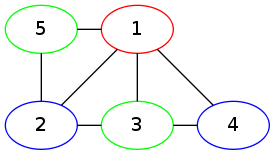
\includegraphics[width=240px]{ex1.png}
    $colors = $
	\begin{tabular}{|c|c|c|c|c|}
	\hline
	1 & 2 & 3 & 2 & 3\\
	\hline
	\end{tabular} \\$ $\\
\end{center}	

\item[c)] \term{Proposez une manière de générer une population initiale diversifiée.} \\

On pourrait générer des colorations aléatoires avec $l$ couleurs pour $l$ allant de $2$ à $n$ (aucun graphe comportant au moins 
une arête n'est $1$-colorable. Selon la fonction de coût choisie, pour certains d'entre eux soit il y aura des sommets non 
coloriés, soit des arêtes conflictuelles. \\

Il conviendra ensuite d'affiner la recherche pour laisser tomber tous les cas supérieur à une borne trouvée, c'est-à-dire que si 
on trouve, par exemple, une $5-coloration$, il est inutile de continuer à chercher ou à garder des $k$-colorations avec $k>5$ (vu 
que le but est de minimiser le nombre de couleurs utilisées).

\item[d)] \term{Proposez deux opérations de mutation différentes. Illustrez-les sur des exemples (graphes et représentations 
codées).} \\

On peut entrevoir les 2 mutations suivantes :
\begin{enumerate}
\item Modifier la couleur d'un seul sommet du graphe. \\
\textbf{\underline{Exemple} :} 

\begin{center}
    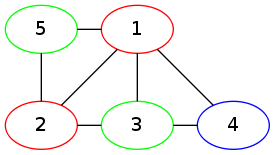
\includegraphics[width=240px]{ex2.png}
    $colors = $
	\begin{tabular}{|c|c|c|c|c|}
	\hline
	1 & 1 & 3 & 2 & 3\\
	\hline
	\end{tabular} \\
	$\Rightarrow$
	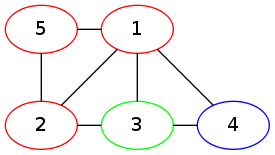
\includegraphics[width=240px]{ex2_2.png}
    $colors = $
	\begin{tabular}{|c|c|c|c|c|}
	\hline
	1 & 1 & 3 & 2 & \dred{1}\\
	\hline
	\end{tabular}  \\$ $\\
\end{center}
\item Modifier la couleur d'un seul sommet étant l'extrêmité d'une arête conflictuelle du graphe.

\textbf{\underline{Exemple} :} 

\begin{center}
    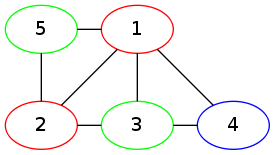
\includegraphics[width=240px]{ex2.png}
    $colors = $
	\begin{tabular}{|c|c|c|c|c|}
	\hline
	1 & 1 & 3 & 2 & 3\\
	\hline
	\end{tabular} \\
	$\Rightarrow$
	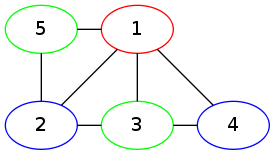
\includegraphics[width=240px]{ex1.png}
    $colors = $
	\begin{tabular}{|c|c|c|c|c|}
	\hline
	1 & \blu{\textbf{2}} & 3 & 2 & 3\\
	\hline
	\end{tabular}  \\$ $\\
\end{center}

Dans ce cas-ci, le résultat est positif car on a résolu un conflit sans en créer un autre, mais il se peut que l'on en crée un 
autre (si on avait remplacé la couleur par du vert au lieu de bleu, par exemple).
\end{enumerate}

\item[e)] \term{Proposez deux opérations de croisement différentes. Illustrez-les sur des exemples (graphes et représentations 
codées).} \\

Voici ces 2 opérations :
\begin{enumerate}
\item on peut croiser 2 parents qui auraient une coloration partiellement correcte, c'est-à-dire que si la solution $s_1$ possède 
une $k$-coloration pour un sous-graphe et la solution $s_2$ une $k$-coloration pour le complémentaire de ce sous-graphe, on 
pourrait croiser les 2 parties légales pour en obtenir une complète, on espère, qui l'est également. \\

\textbf{\underline{Exemple} :} 

\begin{center}
	$s_1 : $
    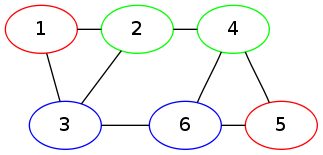
\includegraphics[width=240px]{ex3.png}
    $colors = $
	\begin{tabular}{|c|c|c|c|c|c|}
	\hline
	1 & 3 & 2 & 3 & 1 & 2\\
	\hline
	\end{tabular}\\
	$s_2 :$
	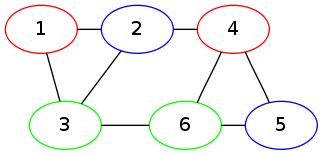
\includegraphics[width=240px]{ex3_2.png}
    $colors = $
	\begin{tabular}{|c|c|c|c|c|c|}
	\hline
	1 & 2 & 3 & 1 & 2 & 3\\
	\hline
	\end{tabular}  \\$ $\\
\end{center}

$s_1$ a une $3-coloration$ légale sur les sommets ${1,2,3}$ et $s_2$ sur ${4,5,6}$, on pourrait alors les croiser pour créer :
\begin{center}
	$s_{result}: $
    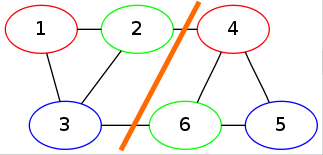
\includegraphics[width=200px]{ex3_3.png}
    $colors = $
	\begin{tabular}{|c|c|c|c|c|c|}
	\hline
	1 & 3 & 2 & 1 & 2 & 3\\
	\hline
	\end{tabular}\\
\end{center}

Dans ce cas $s_{result}$ a une valeur nulle pour la fonction de coût, c'est une solution optimale (vu que le nombre chromatique 
de ce graphe est $3$) mais ce n'est pas toujours le cas. Autrement dit, le croisement peut très bien générer d'autres arêtes 
conflictuelles.

\item D'une manière plus aléatoire, on pourrait croiser 2 parents en prenant les colorations impairs d'un des parents et les 
colorations pairs de l'autre. Il n'y a aucune garantie sur la qualité du résultat, mais cela favorisera normalement la diversité.

Prenons les 2 mêmes $s_1$, $s_2$ que ci-dessus, on pourrait alors créer :

\begin{center}
	$s_{result}: $
    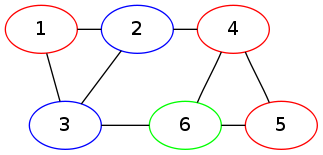
\includegraphics[width=200px]{ex3_4.png}
    $colors = $
	\begin{tabular}{|c|c|c|c|c|c|}
	\hline
	1 & 2 & 2 & 1 & 1 & 3\\
	\hline
	\end{tabular}\\$ $\\$ $\\
\end{center}

\end{enumerate}

\item[f)] \term{Parmi les 4 opérations de variations proposées, pensez-vous qu’il y en ait qui soient mieux adaptées au problème 
? (Justifiez)}

La meilleure, selon moi, est le croisement des 2 parents possédant des $k$-coloration partielle légale. En effet, dans ces sous-
graphes, la $k$-coloration est bonne, les seuls éventuels conflits qu'il restera seront entre 2 noeuds appartenant chacun à un 
des 2 sous-graphes et étant connectés entre eux. Ainsi si cette "zone de connexion" n'est pas énorme, le nombre de conflits 
possible sera très minime, ce qui constituera un bon en avant pour la suite. \\

La mutation de la couleur d'une extrêmité d'une arête conflictuelle me semble très correcte également, en effet, dans le pire des 
cas elle ne modifie rien au problème, car elle résout un conflit pour en créer un autre (voir plus). Dans le meilleur des cas, 
elle enlève un conflit (voir plus).\\

Par contre, la mutation d'un sommet aléatoire n'est vraiment pas aidant car il se peut qu'elle crée énormément de conflits 
supplémentaires (par exemple un noeud bleu avec ses 50 voisins en rouge que l'on recolore en rouge...) mais elle facilite la 
diversité (en effet, par la suite elle pourrait donner lieu a des descendants ou les 50 voisins sont progressivement coloré en 
bleu et résoudre les conflits qui étaient nés à cause de l'emploi de la couleur rouge pour les 50 noeuds). \\

Il en va de même pour le croisement des noeuds pairs/impairs, s'agissant d'une méthode totalement aléatoire, aucun résultat n'est 
garanti, hormis le fait que cela diversifie la population.

\end{enumerate}

\section{Répartition du temps}

\begin{enumerate}
\item entre $2$ et $3$h (difficulté à faire une preuve formelle et à trouver une heuristique admissible et non consistante).
\item $2$h environ, en comptant la mise en page LaTeX.
\item $4$h environ, en comptant la mise en page LaTeX et la création des exemples.
\end{enumerate}

\end{sffamily}\end{document}